% Generated by generate_supplement.py; do not hand-edit.
\documentclass[10pt]{article}
\usepackage[letterpaper,margin=0.65in]{geometry}
\usepackage{newtxtext,newtxmath}
\usepackage{booktabs,longtable,array,pdflscape,graphicx,url}
\usepackage[hidelinks]{hyperref}
\newcolumntype{L}[1]{>{\raggedright\arraybackslash}p{#1}}
\newcolumntype{R}[1]{>{\raggedleft\arraybackslash}p{#1}}
\setlength{\parindent}{0pt}
\setlength{\parskip}{4pt}
\begin{document}
\begin{center}
{\Large\bfseries Companion Results Appendix: GGUF Throughput Prediction\par}
\vspace{4pt}
{\normalsize Protocol-complete two-host evidence for the ICASSP manuscript\par}
\end{center}
\textbf{Status.} This is a locally generated companion appendix. It does not claim publication, archival acceptance, or independent replication.
\section{Scope and cohort}
The source manifest contains 23 GGUF files. Across two hosts, the scored data contain 21 unique files and 33 host--file configurations (27 training and 6 held out). Each configuration has one decode and one prefill observation at each of the 3 measured context depths, for 99 decode and 99 prefill rows. The final protocol selector retains 216 observations from 22 unique files in total: 198 scored rows and 18 reference-probe rows excluded from prediction fits and scores. Probe exclusion is host-specific, so a file used as a probe on one host can be scored on the other.
All exported rows carry the declared protocol fields. The retry decision, however, uses the worst within-run \emph{decode} CV in an invocation. Prefill rows inherit that invocation's protocol metadata but are not gated on their own CV. This distinction matters on RTX 5080, where the noisiest prefill row has 39.19\% CV even though the associated decode-gate CV is 1.35\%.
\begin{center}
\small
\begin{tabular}{llrrrr}
\toprule
Host & Backend & Train cfg. & Test cfg. & Scored decode & Scored prefill\\
\midrule
MacBook M4 Max & BLAS,MTL & 15 & 4 & 57 & 57 \\
RTX 5080 & CUDA & 12 & 2 & 42 & 42 \\
\bottomrule
\end{tabular}
\end{center}
\begin{center}
\small
\begin{tabular}{lrrrrrr}
\toprule
Host & Retried cells & Gate CV med. & Gate CV max & PP CV med. & PP CV max & PP $>3\%$\\
\midrule
MacBook M4 Max & 3 & 1.43 & 3.04 & 1.41 & 4.84 & 7/57 \\
RTX 5080 & 3 & 0.88 & 1.65 & 3.56 & 39.19 & 29/42 \\
\bottomrule
\end{tabular}
\end{center}
Attempted configurations with no successful row are MacBook M4 Max: \nolinkurl{gpt-oss-120b-MXFP4.gguf}. On the MacBook Pro M4 Max, two raw attempts of the one gpt-oss-120B configuration report \texttt{failed to decode prompt batch, res=-3}; these are prompt-batch failures, not demonstrated model-load or out-of-memory failures. Host-specific calibration probes are MacBook M4 Max: \nolinkurl{Qwen3.8-27B-Q8_0.gguf}, \nolinkurl{Qwen3.5-9B-Q8_0.gguf}, \nolinkurl{Qwen3.5-4B-Q8_0.gguf}; RTX 5080: none.
\subsection{Cohort accounting}
Raw records, superseded legacy rows, repeated protocol attempts, selected observations, and scoring exclusions are separated below. A protocol duplicate is a successful protocol row removed by the atomic host--model--phase--depth selector; it is not an additional scored observation.
\begin{center}
\small
\setlength{\tabcolsep}{2.8pt}
\begin{tabular}{lrrrrrrrr}
\toprule
Host & Raw & Failed & Legacy ok & Protocol ok & Dup. removed & Selected & Probes & Scored\\
\midrule
MacBook M4 Max & 278 & 2 & 132 & 144 & 12 & 132 & 18 & 114 \\
RTX 5080 & 84 & 0 & 0 & 84 & 0 & 84 & 0 & 84 \\
\bottomrule
\end{tabular}
\end{center}
\subsection{Excluded reference-probe observations}
These rows complete the 216-observation selected cohort and make the descriptive matched-host and quantization comparisons reproducible. They are reported only as measurements, never as prediction errors.
\begingroup
\small
\setlength{\tabcolsep}{3.5pt}
\renewcommand{\arraystretch}{1.08}
\begin{longtable}{@{}lllrrrrr@{}}
\caption{Selected protocol-complete reference-probe observations excluded from prediction fitting and scoring. Measured throughput and SD are in tokens/s; IDs resolve through Table~\ref{tab:model-id}.}\label{tab:probe-observations}\\
\toprule
Host & ID & Phase & Depth & Measured & SD & CV \% & Attempts \\
\midrule
\endfirsthead
\caption[]{Selected protocol-complete reference-probe observations excluded from prediction fitting and scoring. Measured throughput and SD are in tokens/s; IDs resolve through Table~\ref{tab:model-id}. (continued)}\\
\toprule
Host & ID & Phase & Depth & Measured & SD & CV \% & Attempts \\
\midrule
\endhead
\midrule
\multicolumn{8}{r}{Continued on next page}\\
\endfoot
\bottomrule
\endlastfoot
MacBook M4 Max & M09 & decode & 0 & 77.275 & 0.201 & 0.260 & 1 \\
MacBook M4 Max & M09 & decode & 4,096 & 74.687 & 0.153 & 0.204 & 1 \\
MacBook M4 Max & M09 & decode & 16,384 & 67.270 & 0.341 & 0.507 & 1 \\
MacBook M4 Max & M09 & prefill & 0 & 1553.086 & 1.682 & 0.108 & 1 \\
MacBook M4 Max & M09 & prefill & 4,096 & 1416.098 & 1.799 & 0.127 & 1 \\
MacBook M4 Max & M09 & prefill & 16,384 & 992.403 & 10.398 & 1.048 & 1 \\
MacBook M4 Max & M11 & decode & 0 & 46.499 & 0.380 & 0.818 & 2 \\
MacBook M4 Max & M11 & decode & 4,096 & 45.340 & 0.169 & 0.372 & 2 \\
MacBook M4 Max & M11 & decode & 16,384 & 42.119 & 0.938 & 2.226 & 2 \\
MacBook M4 Max & M11 & prefill & 0 & 865.397 & 0.661 & 0.076 & 2 \\
MacBook M4 Max & M11 & prefill & 4,096 & 784.470 & 4.299 & 0.548 & 2 \\
MacBook M4 Max & M11 & prefill & 16,384 & 560.769 & 14.295 & 2.549 & 2 \\
MacBook M4 Max & M13 & decode & 0 & 14.902 & 0.054 & 0.365 & 1 \\
MacBook M4 Max & M13 & decode & 4,096 & 14.433 & 0.017 & 0.118 & 1 \\
MacBook M4 Max & M13 & decode & 16,384 & 13.575 & 0.092 & 0.680 & 1 \\
MacBook M4 Max & M13 & prefill & 0 & 238.511 & 7.257 & 3.043 & 1 \\
MacBook M4 Max & M13 & prefill & 4,096 & 201.115 & 2.027 & 1.008 & 1 \\
MacBook M4 Max & M13 & prefill & 16,384 & 161.599 & 1.227 & 0.759 & 1 \\
\end{longtable}
\endgroup
\paragraph{Probe-exclusion sensitivity.}
The three Mac Q8 files defined the historical LLM-reference diagnostic. Their exclusion was fixed before the final device-copy analysis and is retained to avoid a post-hoc cohort change. If they are included and B2 is refit, MAPE is 10.46\% over 54 training rows and 13.11\% over 12 held-out rows; the latter is unchanged because all probes are Q8 training files while the test files are Q4. On the original 45 non-probe training rows under this refit, MAPE is 11.06\%.
\section{Aggregate prediction results}
Results are separated by host because fitted efficiency factors are host-specific; a pooled row would weight the unequal host cohorts and is not a cross-system score.
\begin{center}
\small
\begin{tabular}{lllrrrr}
\toprule
Host & Predictor & Split & $n$ & MAPE (\%) & Median (\%) & P90 / max (\%)\\
\midrule
MacBook M4 Max & B0 unfitted (eta=1, total) & train & 45 & 33.57 & 19.37 & 76.47 / 123.27 \\
MacBook M4 Max & B0 unfitted (eta=1, total) & test & 12 & 46.89 & 49.97 & 83.45 / 84.22 \\
MacBook M4 Max & B1 fitted, total params & train & 45 & 15.80 & 3.20 & 70.29 / 76.77 \\
MacBook M4 Max & B1 fitted, total params & test & 12 & 49.36 & 54.66 & 81.90 / 82.74 \\
MacBook M4 Max & B2 fitted, active params (ours) & train & 45 & 10.39 & 2.12 & 26.32 / 78.49 \\
MacBook M4 Max & B2 fitted, active params (ours) & test & 12 & 13.11 & 8.98 & 36.65 / 49.92 \\
RTX 5080 & B0 unfitted (eta=1, total) & train & 36 & 20.27 & 14.47 & 44.15 / 71.19 \\
RTX 5080 & B0 unfitted (eta=1, total) & test & 6 & 41.65 & 40.39 & 81.22 / 81.95 \\
RTX 5080 & B1 fitted, total params & train & 36 & 9.85 & 8.88 & 20.95 / 31.73 \\
RTX 5080 & B1 fitted, total params & test & 6 & 51.85 & 50.81 & 84.50 / 85.11 \\
RTX 5080 & B2 fitted, active params (ours) & train & 36 & 10.12 & 9.34 & 20.95 / 31.73 \\
RTX 5080 & B2 fitted, active params (ours) & test & 6 & 36.15 & 25.79 & 62.41 / 68.96 \\
\midrule
MacBook M4 Max & P1 eta\_p per host & train & 15 & 6.81 & 5.36 & 16.58 / 33.40 \\
MacBook M4 Max & P1 eta\_p per host & test & 4 & 22.68 & 19.16 & 44.95 / 51.25 \\
MacBook M4 Max & P2 eta\_p per host x quant & train & 15 & 4.13 & 0.00 & 15.06 / 25.99 \\
MacBook M4 Max & P2 eta\_p per host x quant & test & 4 & 18.68 & 14.90 & 36.90 / 42.85 \\
RTX 5080 & P1 eta\_p per host & train & 12 & 14.46 & 9.15 & 31.38 / 52.16 \\
RTX 5080 & P1 eta\_p per host & test & 2 & 124.51 & 124.51 & 207.24 / 227.93 \\
RTX 5080 & P2 eta\_p per host x quant & train & 12 & 5.86 & 0.00 & 21.31 / 25.36 \\
RTX 5080 & P2 eta\_p per host x quant & test & 2 & 108.18 & 108.18 & 184.89 / 204.07 \\
\bottomrule
\end{tabular}
\end{center}
Decode summaries use all three context depths. Prefill headline rows use only depth 0, because the stated prefill model has no existing-prefix term; deeper rows are scope diagnostics below.
\subsection{Leave-one-host-out transfer}
B2 transfers the source host's median per-quantization coefficients and substitutes the untouched target host's bandwidth. The target set contains all eligible rows on that host; because most files also occur on the source host, this isolates host/runtime transfer rather than a simultaneous model-and-hardware holdout. Q4\_K\_M is shared; the Mac Q4\_K test file uses the source-wide median fallback. The second variant is the rejected absolute-time output-projection extension.
\begin{center}
\small
\begin{tabular}{llrrrrr}
\toprule
Variant & Target host & Source $n$ & Target $n$ & MAPE & Median & Max\\
\midrule
B2: all target rows & MacBook M4 Max & 36 & 57 & 20.82 & 15.41 & 75.81 \\
B2: all target rows & RTX 5080 & 45 & 42 & 21.69 & 18.75 & 71.53 \\
B2: target test rows & MacBook M4 Max & 36 & 12 & 13.94 & 8.63 & 47.67 \\
B2: target test rows & RTX 5080 & 45 & 6 & 36.70 & 26.18 & 71.53 \\
rejected two-term & MacBook M4 Max & 36 & 57 & 57.06 & 54.22 & 78.57 \\
rejected two-term & RTX 5080 & 45 & 42 & 116.85 & 98.66 & 349.25 \\
\bottomrule
\end{tabular}
\end{center}
For context, target-fitted B2 gives all-row MAPE of 10.96\% on Mac and 13.84\% on RTX. Unlike the untouched-target transfer rows, these comparators mix training rows used to fit the target coefficients with held-out rows.
\begin{center}
\small
\begin{tabular}{lllrrrr}
\toprule
Host & Split & Architecture & $n$ & B0 & B1 & B2\\
\midrule
MacBook M4 Max & train & dense & 36 & 23.21 & 7.14 & 5.66 \\
MacBook M4 Max & train & MoE & 9 & 74.98 & 50.45 & 29.29 \\
MacBook M4 Max & test & dense & 6 & 11.18 & 17.75 & 3.28 \\
MacBook M4 Max & test & MoE & 6 & 82.61 & 80.97 & 22.95 \\
RTX 5080 & train & dense & 33 & 15.73 & 10.57 & 10.57 \\
RTX 5080 & train & MoE & 3 & 70.28 & 1.95 & 5.18 \\
RTX 5080 & test & dense & 3 & 3.54 & 20.40 & 20.40 \\
RTX 5080 & test & MoE & 3 & 79.77 & 83.31 & 51.90 \\
\bottomrule
\end{tabular}
\end{center}
\subsection{Per-layer KV correction}
With each variant refit on training rows, replacing a uniform-global KV denominator by the frozen per-layer metadata produces:
\begin{center}
\small
\begin{tabular}{llrrr}
\toprule
Host & Split & $n$ & Uniform KV MAPE (\%) & Per-layer KV MAPE (\%)\\
\midrule
MacBook M4 Max & train & 45 & 12.68 & 10.39 \\
MacBook M4 Max & test & 12 & 21.23 & 13.11 \\
RTX 5080 & train & 36 & 12.37 & 10.12 \\
RTX 5080 & test & 6 & 37.87 & 36.15 \\
\bottomrule
\end{tabular}
\end{center}
\subsection{Decode context behavior}
All 33 scored host--file configurations slow monotonically from 0 through 16,384 tokens. The normalized rate is each model's throughput divided by its own depth-0 throughput.
\begin{center}
\small
\begin{tabular}{lrrrrrr}
\toprule
Host & Depth & Train $n$ & Test $n$ & Train B2 MAPE & Test B2 MAPE & Median normalized rate\\
\midrule
MacBook M4 Max & 0 & 15 & 4 & 11.30 & 17.86 & 1.000 \\
MacBook M4 Max & 4,096 & 15 & 4 & 7.59 & 12.83 & 0.945 \\
MacBook M4 Max & 16,384 & 15 & 4 & 12.27 & 8.63 & 0.837 \\
RTX 5080 & 0 & 12 & 2 & 10.19 & 44.52 & 1.000 \\
RTX 5080 & 4,096 & 12 & 2 & 4.49 & 38.28 & 0.985 \\
RTX 5080 & 16,384 & 12 & 2 & 15.67 & 25.64 & 0.922 \\
\bottomrule
\end{tabular}
\end{center}
\subsection{Prefill scope diagnostic}
Depth 0 is the primary prefill fit and score. The same fitted coefficients are applied unchanged at larger existing-prefix depths. These errors are prediction errors, distinct from within-run prefill variability; the RTX held-out result is poor even before that distinction is considered.
\begin{center}
\small
\begin{tabular}{llrrrrrr}
\toprule
Host & Split & Depth & $n$ & P1 MAPE & P2 MAPE & P2 median & P2 max\\
\midrule
MacBook M4 Max & train & 0 & 15 & 6.81 & 4.13 & 0.00 & 25.99 \\
MacBook M4 Max & train & 4,096 & 15 & 22.35 & 20.83 & 17.58 & 49.82 \\
MacBook M4 Max & train & 16,384 & 15 & 66.94 & 64.13 & 51.02 & 150.97 \\
MacBook M4 Max & test & 0 & 4 & 22.68 & 18.68 & 14.90 & 42.85 \\
MacBook M4 Max & test & 4,096 & 4 & 40.98 & 33.11 & 29.60 & 55.36 \\
MacBook M4 Max & test & 16,384 & 4 & 86.59 & 76.18 & 73.78 & 132.42 \\
RTX 5080 & train & 0 & 12 & 14.46 & 5.86 & 0.00 & 25.36 \\
RTX 5080 & train & 4,096 & 12 & 19.26 & 12.35 & 8.23 & 32.74 \\
RTX 5080 & train & 16,384 & 12 & 36.13 & 28.56 & 18.19 & 72.26 \\
RTX 5080 & test & 0 & 2 & 124.51 & 108.18 & 108.18 & 204.07 \\
RTX 5080 & test & 4,096 & 2 & 108.39 & 93.23 & 93.23 & 167.57 \\
RTX 5080 & test & 16,384 & 2 & 151.64 & 133.34 & 133.34 & 227.36 \\
\bottomrule
\end{tabular}
\end{center}
\begin{figure}[t]
\centering
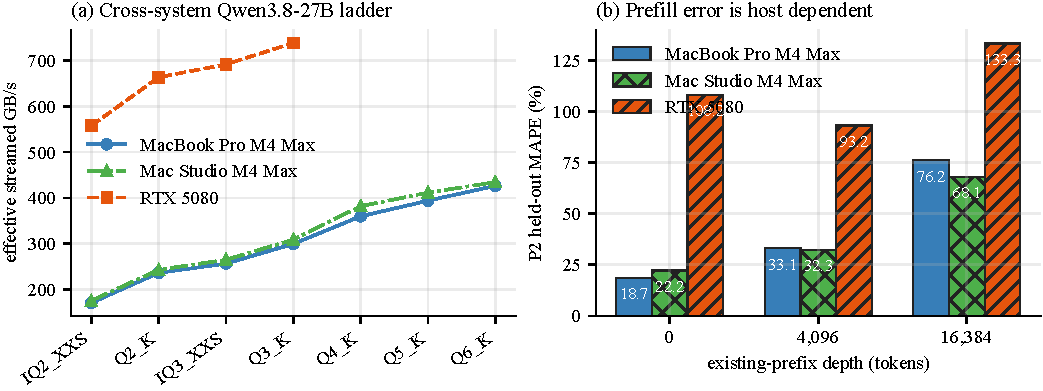
\includegraphics[width=\textwidth]{supplement_summary.pdf}
\caption{Host-separated diagnostics. Left: effective streamed bandwidth for the scored Qwen3.8-27B quantizations at zero prefix; host coverage differs, and IQ2 has 64 layers/26.90B parameters versus 65 layers/27.32B for the other shown files, so the set is a family comparison rather than a strictly identical-network quantization ladder. Right: P2 held-out error when depth-0 coefficients are applied at each existing-prefix depth. The RTX result is not pooled with the Apple result.}
\end{figure}
\begin{landscape}
\section{Selected model metadata}
Tables~\ref{tab:model-id} and~\ref{tab:model-geometry} jointly reproduce every frozen metadata field used for the 22 unique selected files (21 scored and 1 probe-only). Scored host coverage is explicit because the two measurement cohorts are not identical.
\begingroup
\small
\setlength{\tabcolsep}{3.5pt}
\renewcommand{\arraystretch}{1.08}
\begin{longtable}{@{}l l L{0.75in} L{2.7in} L{2.45in} L{0.9in} l r@{}}
\caption{Selected model identity, source, and file size. Sizes are exact bytes; host codes are MB (MacBook M4 Max) and RTX (RTX 5080), and ``probe only'' denotes a file excluded from every prediction fit and score.}\label{tab:model-id}\\
\toprule
ID & Split & Scored host(s) & GGUF filename & Repository & Architecture & Quant. & Bytes \\
\midrule
\endfirsthead
\caption[]{Selected model identity, source, and file size. Sizes are exact bytes; host codes are MB (MacBook M4 Max) and RTX (RTX 5080), and ``probe only'' denotes a file excluded from every prediction fit and score. (continued)}\\
\toprule
ID & Split & Scored host(s) & GGUF filename & Repository & Architecture & Quant. & Bytes \\
\midrule
\endhead
\midrule
\multicolumn{8}{r}{Continued on next page}\\
\endfoot
\bottomrule
\endlastfoot
M01 & train & MB, RTX & \nolinkurl{gemma-4-12b-it-qat-q4_0.gguf} & \nolinkurl{google/gemma-4-12B-it-qat-q4_0-gguf} & gemma4 & Q4\_0 & 6,975,879,296 \\
M02 & train & MB & \nolinkurl{gemma-4-26B-A4B-it-UD-Q4_K_M.gguf} & \nolinkurl{unsloth/gemma-4-26B-A4B-it-GGUF} & gemma4 & Q4\_K\_M & 16,947,541,728 \\
M03 & train & MB, RTX & \nolinkurl{gpt-oss-20b-MXFP4.gguf} & \nolinkurl{ggml-org/gpt-oss-20b-GGUF} & gpt-oss & MXFP4 & 12,109,566,624 \\
M04 & test & MB, RTX & \nolinkurl{inclusionAI_Ling-mini-2.0-Q4_K_M.gguf} & \nolinkurl{bartowski/inclusionAI_Ling-mini-2.0-GGUF} & bailingmoe2 & Q4\_K\_M & 9,941,894,336 \\
M05 & test & MB & \nolinkurl{Muse-Glimmer-30B-UD-Q4_K_XL.gguf} & \nolinkurl{unsloth/Muse-Glimmer-30B-GGUF} & muse-glimmer & Q4\_K & 15,878,222,368 \\
M06 & test & MB & \nolinkurl{Nemotron-3-Nano-30B-A3B-Q4_K_M.gguf} & \nolinkurl{unsloth/Nemotron-3-Nano-30B-A3B-GGUF} & nemotron\_h\_moe & Q4\_K\_M & 24,574,373,664 \\
M07 & test & MB, RTX & \nolinkurl{NVIDIA-Nemotron-3-Nano-4B-Q4_K_M.gguf} & \nolinkurl{lmstudio-community/NVIDIA-Nemotron-3-Nano-4B-GGUF} & nemotron\_h & Q4\_K\_M & 2,837,072,896 \\
M08 & train & MB, RTX & \nolinkurl{Qwen3.5-4B-Q4_K_M.gguf} & \nolinkurl{unsloth/Qwen3.5-4B-GGUF} & qwen35 & Q4\_K\_M & 2,740,937,888 \\
M09 & train & RTX & \nolinkurl{Qwen3.5-4B-Q8_0.gguf} & \nolinkurl{unsloth/Qwen3.5-4B-GGUF} & qwen35 & Q8\_0 & 4,482,403,488 \\
M10 & train & MB, RTX & \nolinkurl{Qwen3.5-9B-Q4_K_M.gguf} & \nolinkurl{unsloth/Qwen3.5-9B-GGUF} & qwen35 & Q4\_K\_M & 5,680,522,464 \\
M11 & train & RTX & \nolinkurl{Qwen3.5-9B-Q8_0.gguf} & \nolinkurl{unsloth/Qwen3.5-9B-GGUF} & qwen35 & Q8\_0 & 9,527,502,048 \\
M12 & train & MB & \nolinkurl{Qwen3.6-35B-A3B-UD-Q4_K_M.gguf} & \nolinkurl{unsloth/Qwen3.6-35B-A3B-GGUF} & qwen35moe & Q4\_K\_M & 22,134,528,992 \\
M13 & probe only & -- & \nolinkurl{Qwen3.8-27B-Q8_0.gguf} & \nolinkurl{unsloth/Qwen3.8-27B-GGUF} & qwen35 & Q8\_0 & 29,047,086,048 \\
M14 & train & MB, RTX & \nolinkurl{Qwen3.8-27B-UD-IQ2_XXS.gguf} & \nolinkurl{unsloth/Qwen3.8-27B-GGUF} & qwen35 & IQ2\_XXS & 7,266,070,528 \\
M15 & train & MB, RTX & \nolinkurl{Qwen3.8-27B-UD-IQ3_XXS.gguf} & \nolinkurl{unsloth/Qwen3.8-27B-GGUF} & qwen35 & IQ3\_XXS & 10,934,860,704 \\
M16 & train & MB, RTX & \nolinkurl{Qwen3.8-27B-UD-Q2_K_XL.gguf} & \nolinkurl{unsloth/Qwen3.8-27B-GGUF} & qwen35 & Q2\_K & 9,828,981,664 \\
M17 & train & MB, RTX & \nolinkurl{Qwen3.8-27B-UD-Q3_K_XL.gguf} & \nolinkurl{unsloth/Qwen3.8-27B-GGUF} & qwen35 & Q3\_K & 13,146,393,504 \\
M18 & train & MB & \nolinkurl{Qwen3.8-27B-UD-Q4_K_XL.gguf} & \nolinkurl{unsloth/Qwen3.8-27B-GGUF} & qwen35 & Q4\_K & 17,559,178,144 \\
M19 & train & MB & \nolinkurl{Qwen3.8-27B-UD-Q5_K_XL.gguf} & \nolinkurl{unsloth/Qwen3.8-27B-GGUF} & qwen35 & Q5\_K & 20,876,938,144 \\
M20 & train & MB & \nolinkurl{Qwen3.8-27B-UD-Q6_K_XL.gguf} & \nolinkurl{unsloth/Qwen3.8-27B-GGUF} & qwen35 & Q6\_K & 25,299,061,664 \\
M21 & train & MB, RTX & \nolinkurl{SmolLM3-Q4_K_M.gguf} & \nolinkurl{ggml-org/SmolLM3-3B-GGUF} & smollm3 & Q4\_K\_M & 1,915,305,312 \\
M22 & train & MB, RTX & \nolinkurl{SmolLM3-Q8_0.gguf} & \nolinkurl{ggml-org/SmolLM3-3B-GGUF} & smollm3 & Q8\_0 & 3,275,574,624 \\
\end{longtable}
\endgroup
\end{landscape}
\begin{landscape}
\begingroup
\small
\setlength{\tabcolsep}{3.5pt}
\renewcommand{\arraystretch}{1.08}
\begin{longtable}{@{}l r r r r r r r r r r r r@{}}
\caption{Selected model geometry. KV columns are exact bytes at the measured depths; $k/E$ is routed/total experts.}\label{tab:model-geometry}\\
\toprule
ID & Total P & Active P & Active \% & Layers & Width & Vocab. & KV heads & Head dim. & Used/all & KV@0 & KV@4096 & KV@16384 \\
\midrule
\endfirsthead
\caption[]{Selected model geometry. KV columns are exact bytes at the measured depths; $k/E$ is routed/total experts. (continued)}\\
\toprule
ID & Total P & Active P & Active \% & Layers & Width & Vocab. & KV heads & Head dim. & Used/all & KV@0 & KV@4096 & KV@16384 \\
\midrule
\endhead
\midrule
\multicolumn{13}{r}{Continued on next page}\\
\endfoot
\bottomrule
\endlastfoot
M01 & 11,907,350,576 & 11,907,350,576 & 100.0 & 48 & 3,840 & 262,144 & 8 & 512 & -- & 0 & 738,197,504 & 939,524,096 \\
M02 & 25,233,142,046 & 3,822,527,246 & 15.1 & 30 & 2,816 & 262,144 & 8 & 512 & 8/128 & 0 & 503,316,480 & 754,974,720 \\
M03 & 20,914,757,184 & 4,187,440,704 & 20.0 & 24 & 2,880 & 201,088 & 8 & 64 & 4/32 & 0 & 201,326,592 & 805,306,368 \\
M04 & 16,255,643,392 & 1,432,973,056 & 8.8 & 20 & 2,048 & 157,184 & 4 & 128 & 8/256 & 0 & 167,772,160 & 671,088,640 \\
M05 & 27,854,794,240 & 27,854,794,240 & 100.0 & 52 & 6,656 & 202,048 & 2 & 128 & -- & 0 & 218,103,808 & 872,415,232 \\
M06 & 31,577,940,288 & 3,580,076,352 & 11.3 & 52 & 2,688 & 131,072 & 2 & 128 & 6/128 & 397,934,592 & 423,100,416 & 498,597,888 \\
M07 & 3,973,556,832 & 3,973,556,832 & 100.0 & 42 & 3,136 & 131,072 & 8 & 128 & -- & 616,366,080 & 683,474,944 & 884,801,536 \\
M08 & 4,205,751,296 & 4,205,751,296 & 100.0 & 32 & 2,560 & 248,320 & 4 & 256 & -- & 0 & 536,870,912 & 2,147,483,648 \\
M09 & 4,205,751,296 & 4,205,751,296 & 100.0 & 32 & 2,560 & 248,320 & 4 & 256 & -- & 0 & 536,870,912 & 2,147,483,648 \\
M10 & 8,953,803,264 & 8,953,803,264 & 100.0 & 32 & 4,096 & 248,320 & 4 & 256 & -- & 0 & 536,870,912 & 2,147,483,648 \\
M11 & 8,953,803,264 & 8,953,803,264 & 100.0 & 32 & 4,096 & 248,320 & 4 & 256 & -- & 0 & 536,870,912 & 2,147,483,648 \\
M12 & 34,660,610,688 & 3,454,988,928 & 10.0 & 40 & 2,048 & 248,320 & 2 & 256 & 8/256 & 0 & 335,544,320 & 1,342,177,280 \\
M13 & 27,320,697,856 & 27,320,697,856 & 100.0 & 65 & 5,120 & 248,320 & 4 & 256 & -- & 0 & 1,090,519,040 & 4,362,076,160 \\
M14 & 26,895,998,464 & 26,895,998,464 & 100.0 & 64 & 5,120 & 248,320 & 4 & 256 & -- & 0 & 1,073,741,824 & 4,294,967,296 \\
M15 & 27,320,697,856 & 27,320,697,856 & 100.0 & 65 & 5,120 & 248,320 & 4 & 256 & -- & 0 & 1,090,519,040 & 4,362,076,160 \\
M16 & 27,320,697,856 & 27,320,697,856 & 100.0 & 65 & 5,120 & 248,320 & 4 & 256 & -- & 0 & 1,090,519,040 & 4,362,076,160 \\
M17 & 27,320,697,856 & 27,320,697,856 & 100.0 & 65 & 5,120 & 248,320 & 4 & 256 & -- & 0 & 1,090,519,040 & 4,362,076,160 \\
M18 & 27,320,697,856 & 27,320,697,856 & 100.0 & 65 & 5,120 & 248,320 & 4 & 256 & -- & 0 & 1,090,519,040 & 4,362,076,160 \\
M19 & 27,320,697,856 & 27,320,697,856 & 100.0 & 65 & 5,120 & 248,320 & 4 & 256 & -- & 0 & 1,090,519,040 & 4,362,076,160 \\
M20 & 27,320,697,856 & 27,320,697,856 & 100.0 & 65 & 5,120 & 248,320 & 4 & 256 & -- & 0 & 1,090,519,040 & 4,362,076,160 \\
M21 & 3,075,098,624 & 3,075,098,624 & 100.0 & 36 & 2,048 & 128,256 & 4 & 128 & -- & 0 & 301,989,888 & 1,207,959,552 \\
M22 & 3,075,098,624 & 3,075,098,624 & 100.0 & 36 & 2,048 & 128,256 & 4 & 128 & -- & 0 & 301,989,888 & 1,207,959,552 \\
\end{longtable}
\endgroup
\end{landscape}
\begin{landscape}
\section{All scored decode observations}
These are the 99 rows exported by \nolinkurl{results/predictions.csv}. Throughput is tokens/s; APE is absolute percentage error. Rows are ordered by host, split, model ID, and depth.
\begingroup
\small
\setlength{\tabcolsep}{3.5pt}
\renewcommand{\arraystretch}{1.08}
\begin{longtable}{@{}l l l r r r r r r r@{}}
\caption{Protocol-complete decode measurements and B2 predictions. The retry gate uses the worst decode CV in each host--file invocation. Pre-load is the macOS one-minute POSIX load average or, on Windows, busy-logical-CPU equivalents; it is meaningful within a host but not comparable across hosts.}\label{tab:decode-rows}\\
\toprule
Host & ID & Split & Depth & Measured & B2 & APE \% & Row CV \% & Load & Attempts \\
\midrule
\endfirsthead
\caption[]{Protocol-complete decode measurements and B2 predictions. The retry gate uses the worst decode CV in each host--file invocation. Pre-load is the macOS one-minute POSIX load average or, on Windows, busy-logical-CPU equivalents; it is meaningful within a host but not comparable across hosts. (continued)}\\
\toprule
Host & ID & Split & Depth & Measured & B2 & APE \% & Row CV \% & Load & Attempts \\
\midrule
\endhead
\midrule
\multicolumn{10}{r}{Continued on next page}\\
\endfoot
\bottomrule
\endlastfoot
MacBook M4 Max & M01 & train & 0 & 54.28 & 54.28 & 0.00 & 0.42 & 15.79 & 1 \\
MacBook M4 Max & M01 & train & 4,096 & 49.91 & 49.08 & 1.65 & 0.55 & 15.79 & 1 \\
MacBook M4 Max & M01 & train & 16,384 & 45.34 & 47.84 & 5.50 & 1.54 & 15.79 & 1 \\
MacBook M4 Max & M02 & train & 0 & 89.15 & 124.01 & 39.11 & 0.15 & 16.58 & 1 \\
MacBook M4 Max & M02 & train & 4,096 & 82.91 & 103.69 & 25.07 & 0.42 & 16.58 & 1 \\
MacBook M4 Max & M02 & train & 16,384 & 75.37 & 95.83 & 27.15 & 0.44 & 16.58 & 1 \\
MacBook M4 Max & M03 & train & 0 & 124.28 & 128.17 & 3.13 & 0.29 & 11.83 & 1 \\
MacBook M4 Max & M03 & train & 4,096 & 118.34 & 118.34 & 0.00 & 0.19 & 11.83 & 1 \\
MacBook M4 Max & M03 & train & 16,384 & 102.83 & 96.21 & 6.43 & 0.67 & 11.83 & 1 \\
MacBook M4 Max & M08 & train & 0 & 101.64 & 116.16 & 14.29 & 0.16 & 8.19 & 1 \\
MacBook M4 Max & M08 & train & 4,096 & 97.13 & 97.13 & 0.00 & 0.28 & 8.19 & 1 \\
MacBook M4 Max & M08 & train & 16,384 & 85.05 & 65.13 & 23.42 & 1.25 & 8.19 & 1 \\
MacBook M4 Max & M10 & train & 0 & 66.64 & 56.05 & 15.90 & 1.00 & 8.30 & 1 \\
MacBook M4 Max & M10 & train & 4,096 & 62.95 & 51.21 & 18.65 & 1.81 & 8.30 & 1 \\
MacBook M4 Max & M10 & train & 16,384 & 56.62 & 40.67 & 28.17 & 2.81 & 8.30 & 1 \\
MacBook M4 Max & M12 & train & 0 & 80.85 & 144.30 & 78.49 & 0.29 & 15.62 & 1 \\
MacBook M4 Max & M12 & train & 4,096 & 78.38 & 125.26 & 59.81 & 0.24 & 15.62 & 1 \\
MacBook M4 Max & M12 & train & 16,384 & 72.10 & 89.72 & 24.44 & 1.12 & 15.62 & 1 \\
MacBook M4 Max & M14 & train & 0 & 23.56 & 23.56 & 0.00 & 1.20 & 16.52 & 1 \\
MacBook M4 Max & M14 & train & 4,096 & 20.41 & 20.53 & 0.59 & 2.70 & 16.52 & 1 \\
MacBook M4 Max & M14 & train & 16,384 & 19.71 & 14.81 & 24.88 & 1.72 & 16.52 & 1 \\
MacBook M4 Max & M15 & train & 0 & 23.49 & 24.42 & 3.94 & 1.09 & 14.84 & 1 \\
MacBook M4 Max & M15 & train & 4,096 & 22.20 & 22.20 & 0.00 & 1.59 & 14.84 & 1 \\
MacBook M4 Max & M15 & train & 16,384 & 19.63 & 17.45 & 11.07 & 1.65 & 14.84 & 1 \\
MacBook M4 Max & M16 & train & 0 & 24.08 & 25.71 & 6.75 & 1.90 & 11.04 & 1 \\
MacBook M4 Max & M16 & train & 4,096 & 23.14 & 23.14 & 0.00 & 2.39 & 11.04 & 1 \\
MacBook M4 Max & M16 & train & 16,384 & 21.30 & 17.81 & 16.41 & 1.65 & 11.04 & 1 \\
MacBook M4 Max & M17 & train & 0 & 22.80 & 23.29 & 2.12 & 2.60 & 11.42 & 3 \\
MacBook M4 Max & M17 & train & 4,096 & 21.89 & 21.50 & 1.75 & 0.91 & 11.42 & 3 \\
MacBook M4 Max & M17 & train & 16,384 & 17.49 & 17.49 & 0.00 & 2.94 & 11.42 & 3 \\
MacBook M4 Max & M18 & train & 0 & 20.50 & 20.92 & 2.05 & 2.11 & 13.06 & 3 \\
MacBook M4 Max & M18 & train & 4,096 & 19.70 & 19.70 & 0.00 & 1.97 & 13.06 & 3 \\
MacBook M4 Max & M18 & train & 16,384 & 16.77 & 16.76 & 0.10 & 1.47 & 13.06 & 3 \\
MacBook M4 Max & M19 & train & 0 & 18.88 & 19.13 & 1.31 & 1.57 & 17.66 & 1 \\
MacBook M4 Max & M19 & train & 4,096 & 18.33 & 18.18 & 0.83 & 2.21 & 17.66 & 1 \\
MacBook M4 Max & M19 & train & 16,384 & 15.82 & 15.82 & 0.00 & 2.67 & 17.66 & 1 \\
MacBook M4 Max & M20 & train & 0 & 16.86 & 16.86 & 0.00 & 0.37 & 17.18 & 1 \\
MacBook M4 Max & M20 & train & 4,096 & 15.92 & 16.16 & 1.50 & 1.42 & 17.18 & 1 \\
MacBook M4 Max & M20 & train & 16,384 & 14.97 & 14.38 & 3.96 & 0.92 & 17.18 & 1 \\
MacBook M4 Max & M21 & train & 0 & 169.50 & 166.23 & 1.93 & 0.46 & 13.91 & 1 \\
MacBook M4 Max & M21 & train & 4,096 & 149.47 & 143.59 & 3.93 & 0.31 & 13.91 & 1 \\
MacBook M4 Max & M21 & train & 16,384 & 115.22 & 101.94 & 11.53 & 0.40 & 13.91 & 1 \\
MacBook M4 Max & M22 & train & 0 & 118.87 & 119.53 & 0.55 & 0.40 & 13.92 & 1 \\
MacBook M4 Max & M22 & train & 4,096 & 109.44 & 109.44 & 0.00 & 0.41 & 13.92 & 1 \\
MacBook M4 Max & M22 & train & 16,384 & 88.22 & 87.32 & 1.01 & 1.00 & 13.92 & 1 \\
MacBook M4 Max & M04 & test & 0 & 242.33 & 363.29 & 49.92 & 1.24 & 11.64 & 1 \\
MacBook M4 Max & M04 & test & 4,096 & 219.67 & 304.92 & 38.81 & 0.84 & 11.64 & 1 \\
MacBook M4 Max & M04 & test & 16,384 & 175.60 & 205.75 & 17.17 & 0.37 & 11.64 & 1 \\
MacBook M4 Max & M05 & test & 0 & 26.23 & 23.14 & 11.81 & 1.92 & 8.93 & 3 \\
MacBook M4 Max & M05 & test & 4,096 & 23.30 & 22.82 & 2.05 & 2.13 & 8.93 & 3 \\
MacBook M4 Max & M05 & test & 16,384 & 22.55 & 21.93 & 2.74 & 3.03 & 8.93 & 3 \\
MacBook M4 Max & M06 & test & 0 & 92.12 & 100.00 & 8.55 & 0.30 & 10.01 & 1 \\
MacBook M4 Max & M06 & test & 4,096 & 90.68 & 99.21 & 9.41 & 0.49 & 10.01 & 1 \\
MacBook M4 Max & M06 & test & 16,384 & 85.16 & 96.93 & 13.83 & 0.68 & 10.01 & 1 \\
MacBook M4 Max & M07 & test & 0 & 93.29 & 92.19 & 1.18 & 0.30 & 8.78 & 1 \\
MacBook M4 Max & M07 & test & 4,096 & 91.41 & 90.44 & 1.07 & 0.10 & 8.78 & 1 \\
MacBook M4 Max & M07 & test & 16,384 & 84.86 & 85.55 & 0.80 & 0.42 & 8.78 & 1 \\
RTX 5080 & M01 & train & 0 & 98.27 & 104.03 & 5.86 & 0.31 & 3.58 & 1 \\
RTX 5080 & M01 & train & 4,096 & 94.08 & 94.08 & 0.00 & 0.64 & 3.58 & 1 \\
RTX 5080 & M01 & train & 16,384 & 92.53 & 91.68 & 0.91 & 0.45 & 3.58 & 1 \\
RTX 5080 & M03 & train & 0 & 229.65 & 236.51 & 2.99 & 0.48 & 8.58 & 2 \\
RTX 5080 & M03 & train & 4,096 & 218.37 & 218.37 & 0.00 & 0.54 & 8.58 & 2 \\
RTX 5080 & M03 & train & 16,384 & 203.03 & 177.54 & 12.56 & 1.58 & 8.58 & 2 \\
RTX 5080 & M08 & train & 0 & 202.01 & 241.17 & 19.39 & 0.33 & 1.02 & 1 \\
RTX 5080 & M08 & train & 4,096 & 198.97 & 201.67 & 1.36 & 0.50 & 1.02 & 1 \\
RTX 5080 & M08 & train & 16,384 & 181.22 & 135.22 & 25.38 & 0.52 & 1.02 & 1 \\
RTX 5080 & M09 & train & 0 & 147.62 & 163.32 & 10.64 & 0.15 & 1.60 & 1 \\
RTX 5080 & M09 & train & 4,096 & 145.85 & 145.85 & 0.00 & 0.50 & 1.60 & 1 \\
RTX 5080 & M09 & train & 16,384 & 136.04 & 110.42 & 18.83 & 0.34 & 1.60 & 1 \\
RTX 5080 & M10 & train & 0 & 132.95 & 116.37 & 12.47 & 0.15 & 1.66 & 1 \\
RTX 5080 & M10 & train & 4,096 & 131.63 & 106.32 & 19.23 & 0.43 & 1.66 & 1 \\
RTX 5080 & M10 & train & 16,384 & 123.69 & 84.44 & 31.73 & 0.43 & 1.66 & 1 \\
RTX 5080 & M11 & train & 0 & 88.98 & 76.84 & 13.65 & 0.09 & 1.47 & 1 \\
RTX 5080 & M11 & train & 4,096 & 88.23 & 72.74 & 17.55 & 0.23 & 1.47 & 1 \\
RTX 5080 & M11 & train & 16,384 & 84.85 & 62.70 & 26.10 & 0.24 & 1.47 & 1 \\
RTX 5080 & M14 & train & 0 & 76.76 & 86.74 & 13.01 & 0.33 & 11.26 & 2 \\
RTX 5080 & M14 & train & 4,096 & 75.58 & 75.58 & 0.00 & 0.49 & 11.26 & 2 \\
RTX 5080 & M14 & train & 16,384 & 70.36 & 54.52 & 22.51 & 1.39 & 11.26 & 2 \\
RTX 5080 & M15 & train & 0 & 63.24 & 68.69 & 8.62 & 0.28 & 14.78 & 1 \\
RTX 5080 & M15 & train & 4,096 & 62.46 & 62.46 & 0.00 & 0.41 & 14.78 & 1 \\
RTX 5080 & M15 & train & 16,384 & 58.63 & 49.10 & 16.25 & 1.50 & 14.78 & 1 \\
RTX 5080 & M16 & train & 0 & 67.48 & 73.66 & 9.15 & 0.30 & 12.10 & 1 \\
RTX 5080 & M16 & train & 4,096 & 66.30 & 66.30 & 0.00 & 0.41 & 12.10 & 1 \\
RTX 5080 & M16 & train & 16,384 & 62.22 & 51.02 & 18.00 & 1.65 & 12.10 & 1 \\
RTX 5080 & M17 & train & 0 & 56.15 & 60.10 & 7.02 & 0.22 & 7.74 & 1 \\
RTX 5080 & M17 & train & 4,096 & 55.49 & 55.49 & 0.00 & 0.36 & 7.74 & 1 \\
RTX 5080 & M17 & train & 16,384 & 52.65 & 45.12 & 14.30 & 1.02 & 7.74 & 1 \\
RTX 5080 & M21 & train & 0 & 306.16 & 345.13 & 12.73 & 0.49 & 1.41 & 1 \\
RTX 5080 & M21 & train & 4,096 & 272.17 & 298.13 & 9.54 & 0.74 & 1.41 & 1 \\
RTX 5080 & M21 & train & 16,384 & 211.65 & 211.65 & 0.00 & 0.48 & 1.41 & 1 \\
RTX 5080 & M22 & train & 0 & 209.46 & 223.49 & 6.70 & 0.19 & 0.70 & 1 \\
RTX 5080 & M22 & train & 4,096 & 192.60 & 204.63 & 6.24 & 0.33 & 0.70 & 1 \\
RTX 5080 & M22 & train & 16,384 & 160.88 & 163.28 & 1.49 & 0.29 & 0.70 & 1 \\
RTX 5080 & M04 & test & 0 & 446.42 & 754.26 & 68.96 & 0.76 & 2.05 & 1 \\
RTX 5080 & M04 & test & 4,096 & 406.19 & 633.07 & 55.85 & 1.35 & 2.05 & 1 \\
RTX 5080 & M04 & test & 16,384 & 326.38 & 427.17 & 30.88 & 1.04 & 2.05 & 1 \\
RTX 5080 & M07 & test & 0 & 239.52 & 191.41 & 20.09 & 0.41 & 1.86 & 2 \\
RTX 5080 & M07 & test & 4,096 & 236.79 & 187.76 & 20.70 & 0.29 & 1.86 & 2 \\
RTX 5080 & M07 & test & 16,384 & 223.15 & 177.61 & 20.41 & 1.01 & 1.86 & 2 \\
\end{longtable}
\endgroup
\end{landscape}
\begin{landscape}
\section{All scored prefill observations}
These are the 99 rows exported by \nolinkurl{results/predictions_prefill.csv}. P1 has one host coefficient; P2 has one host-by-quantization coefficient. Both are fit only at depth 0. The row CV column is reported rather than used as an inclusion filter.
\begingroup
\small
\setlength{\tabcolsep}{3.5pt}
\renewcommand{\arraystretch}{1.08}
\begin{longtable}{@{}l l l r l r r r r r r@{}}
\caption{Protocol-complete prefill measurements and predictions. The retry decision was decode-gated, not prefill-gated; depth-0 rows are the primary evaluation and larger depths are scope diagnostics.}\label{tab:prefill-rows}\\
\toprule
Host & ID & Split & Depth & Scope & Measured & P1 & P1 APE & P2 & P2 APE & Row CV \% \\
\midrule
\endfirsthead
\caption[]{Protocol-complete prefill measurements and predictions. The retry decision was decode-gated, not prefill-gated; depth-0 rows are the primary evaluation and larger depths are scope diagnostics. (continued)}\\
\toprule
Host & ID & Split & Depth & Scope & Measured & P1 & P1 APE & P2 & P2 APE & Row CV \% \\
\midrule
\endhead
\midrule
\multicolumn{11}{r}{Continued on next page}\\
\endfoot
\bottomrule
\endlastfoot
MacBook M4 Max & M01 & train & 0 & \textbf{primary} & 589.73 & 547.32 & 7.19 & 589.73 & 0.00 & 0.05 \\
MacBook M4 Max & M01 & train & 4,096 & diagnostic & 491.90 & 547.32 & 11.27 & 589.73 & 19.89 & 1.01 \\
MacBook M4 Max & M01 & train & 16,384 & diagnostic & 382.76 & 547.32 & 42.99 & 589.73 & 54.07 & 3.47 \\
MacBook M4 Max & M02 & train & 0 & \textbf{primary} & 1418.29 & 1704.93 & 20.21 & 1610.29 & 13.54 & 0.38 \\
MacBook M4 Max & M02 & train & 4,096 & diagnostic & 1145.69 & 1704.93 & 48.81 & 1610.29 & 40.55 & 2.81 \\
MacBook M4 Max & M02 & train & 16,384 & diagnostic & 741.02 & 1704.93 & 130.08 & 1610.29 & 117.31 & 2.63 \\
MacBook M4 Max & M03 & train & 0 & \textbf{primary} & 1589.84 & 1556.35 & 2.11 & 1589.84 & 0.00 & 0.27 \\
MacBook M4 Max & M03 & train & 4,096 & diagnostic & 1372.89 & 1556.35 & 13.36 & 1589.84 & 15.80 & 2.79 \\
MacBook M4 Max & M03 & train & 16,384 & diagnostic & 848.96 & 1556.35 & 83.33 & 1589.84 & 87.27 & 0.72 \\
MacBook M4 Max & M08 & train & 0 & \textbf{primary} & 1463.56 & 1549.58 & 5.88 & 1463.56 & 0.00 & 0.07 \\
MacBook M4 Max & M08 & train & 4,096 & diagnostic & 1310.45 & 1549.58 & 18.25 & 1463.56 & 11.68 & 0.40 \\
MacBook M4 Max & M08 & train & 16,384 & diagnostic & 941.78 & 1549.58 & 64.54 & 1463.56 & 55.40 & 0.89 \\
MacBook M4 Max & M10 & train & 0 & \textbf{primary} & 819.16 & 727.86 & 11.14 & 687.46 & 16.08 & 0.13 \\
MacBook M4 Max & M10 & train & 4,096 & diagnostic & 727.07 & 727.86 & 0.11 & 687.46 & 5.45 & 0.39 \\
MacBook M4 Max & M10 & train & 16,384 & diagnostic & 564.60 & 727.86 & 28.92 & 687.46 & 21.76 & 1.59 \\
MacBook M4 Max & M12 & train & 0 & \textbf{primary} & 1414.02 & 1886.30 & 33.40 & 1781.59 & 25.99 & 0.67 \\
MacBook M4 Max & M12 & train & 4,096 & diagnostic & 1189.17 & 1886.30 & 58.62 & 1781.59 & 49.82 & 1.38 \\
MacBook M4 Max & M12 & train & 16,384 & diagnostic & 880.48 & 1886.30 & 114.24 & 1781.59 & 102.34 & 1.39 \\
MacBook M4 Max & M14 & train & 0 & \textbf{primary} & 239.52 & 242.31 & 1.17 & 239.52 & 0.00 & 2.73 \\
MacBook M4 Max & M14 & train & 4,096 & diagnostic & 196.04 & 242.31 & 23.60 & 239.52 & 22.18 & 0.31 \\
MacBook M4 Max & M14 & train & 16,384 & diagnostic & 158.60 & 242.31 & 52.78 & 239.52 & 51.02 & 1.33 \\
MacBook M4 Max & M15 & train & 0 & \textbf{primary} & 238.54 & 238.54 & 0.00 & 238.54 & 0.00 & 2.42 \\
MacBook M4 Max & M15 & train & 4,096 & diagnostic & 203.40 & 238.54 & 17.28 & 238.54 & 17.28 & 1.81 \\
MacBook M4 Max & M15 & train & 16,384 & diagnostic & 172.91 & 238.54 & 37.96 & 238.54 & 37.96 & 1.74 \\
MacBook M4 Max & M16 & train & 0 & \textbf{primary} & 235.14 & 238.54 & 1.45 & 235.14 & 0.00 & 1.72 \\
MacBook M4 Max & M16 & train & 4,096 & diagnostic & 207.61 & 238.54 & 14.90 & 235.14 & 13.26 & 2.63 \\
MacBook M4 Max & M16 & train & 16,384 & diagnostic & 180.12 & 238.54 & 32.43 & 235.14 & 30.54 & 1.42 \\
MacBook M4 Max & M17 & train & 0 & \textbf{primary} & 241.51 & 238.54 & 1.23 & 241.51 & 0.00 & 2.59 \\
MacBook M4 Max & M17 & train & 4,096 & diagnostic & 202.71 & 238.54 & 17.67 & 241.51 & 19.14 & 0.93 \\
MacBook M4 Max & M17 & train & 16,384 & diagnostic & 164.64 & 238.54 & 44.89 & 241.51 & 46.69 & 2.76 \\
MacBook M4 Max & M18 & train & 0 & \textbf{primary} & 224.91 & 238.54 & 6.06 & 224.91 & 0.00 & 3.91 \\
MacBook M4 Max & M18 & train & 4,096 & diagnostic & 191.29 & 238.54 & 24.70 & 224.91 & 17.58 & 0.80 \\
MacBook M4 Max & M18 & train & 16,384 & diagnostic & 162.37 & 238.54 & 46.91 & 224.91 & 38.52 & 2.61 \\
MacBook M4 Max & M19 & train & 0 & \textbf{primary} & 225.20 & 238.54 & 5.92 & 225.20 & 0.00 & 2.87 \\
MacBook M4 Max & M19 & train & 4,096 & diagnostic & 196.00 & 238.54 & 21.70 & 225.20 & 14.90 & 2.15 \\
MacBook M4 Max & M19 & train & 16,384 & diagnostic & 174.79 & 238.54 & 36.47 & 225.20 & 28.84 & 1.41 \\
MacBook M4 Max & M20 & train & 0 & \textbf{primary} & 239.03 & 238.54 & 0.20 & 239.03 & 0.00 & 2.54 \\
MacBook M4 Max & M20 & train & 4,096 & diagnostic & 208.07 & 238.54 & 14.64 & 239.03 & 14.88 & 2.22 \\
MacBook M4 Max & M20 & train & 16,384 & diagnostic & 181.38 & 238.54 & 31.52 & 239.03 & 31.78 & 1.35 \\
MacBook M4 Max & M21 & train & 0 & \textbf{primary} & 2135.94 & 2119.33 & 0.78 & 2001.68 & 6.29 & 0.04 \\
MacBook M4 Max & M21 & train & 4,096 & diagnostic & 1653.76 & 2119.33 & 28.15 & 2001.68 & 21.04 & 2.82 \\
MacBook M4 Max & M21 & train & 16,384 & diagnostic & 965.07 & 2119.33 & 119.60 & 2001.68 & 107.41 & 1.34 \\
MacBook M4 Max & M22 & train & 0 & \textbf{primary} & 2239.31 & 2119.33 & 5.36 & 2239.31 & 0.00 & 0.12 \\
MacBook M4 Max & M22 & train & 4,096 & diagnostic & 1735.34 & 2119.33 & 22.13 & 2239.31 & 29.04 & 0.12 \\
MacBook M4 Max & M22 & train & 16,384 & diagnostic & 892.27 & 2119.33 & 137.52 & 2239.31 & 150.97 & 1.34 \\
MacBook M4 Max & M04 & test & 0 & \textbf{primary} & 4208.20 & 4547.98 & 8.07 & 4295.53 & 2.08 & 0.42 \\
MacBook M4 Max & M04 & test & 4,096 & diagnostic & 3300.39 & 4547.98 & 37.80 & 4295.53 & 30.15 & 0.62 \\
MacBook M4 Max & M04 & test & 16,384 & diagnostic & 1848.16 & 4547.98 & 146.08 & 4295.53 & 132.42 & 1.94 \\
MacBook M4 Max & M05 & test & 0 & \textbf{primary} & 236.65 & 233.97 & 1.13 & 220.60 & 6.78 & 3.52 \\
MacBook M4 Max & M05 & test & 4,096 & diagnostic & 187.15 & 233.97 & 25.01 & 220.60 & 17.87 & 3.95 \\
MacBook M4 Max & M05 & test & 16,384 & diagnostic & 176.87 & 233.97 & 32.28 & 220.60 & 24.72 & 1.62 \\
MacBook M4 Max & M06 & test & 0 & \textbf{primary} & 1203.59 & 1820.39 & 51.25 & 1719.34 & 42.85 & 0.45 \\
MacBook M4 Max & M06 & test & 4,096 & diagnostic & 1106.68 & 1820.39 & 64.49 & 1719.34 & 55.36 & 3.64 \\
MacBook M4 Max & M06 & test & 16,384 & diagnostic & 895.52 & 1820.39 & 103.28 & 1719.34 & 91.99 & 1.19 \\
MacBook M4 Max & M07 & test & 0 & \textbf{primary} & 1259.18 & 1640.13 & 30.25 & 1549.08 & 23.02 & 4.84 \\
MacBook M4 Max & M07 & test & 4,096 & diagnostic & 1200.41 & 1640.13 & 36.63 & 1549.08 & 29.05 & 3.30 \\
MacBook M4 Max & M07 & test & 16,384 & diagnostic & 995.75 & 1640.13 & 64.71 & 1549.08 & 55.57 & 1.37 \\
RTX 5080 & M01 & train & 0 & \textbf{primary} & 5624.55 & 4619.99 & 17.86 & 5624.55 & 0.00 & 5.17 \\
RTX 5080 & M01 & train & 4,096 & diagnostic & 5030.69 & 4619.99 & 8.16 & 5624.55 & 11.80 & 3.92 \\
RTX 5080 & M01 & train & 16,384 & diagnostic & 4336.80 & 4619.99 & 6.53 & 5624.55 & 29.69 & 2.60 \\
RTX 5080 & M03 & train & 0 & \textbf{primary} & 8633.84 & 13137.34 & 52.16 & 8633.84 & 0.00 & 3.75 \\
RTX 5080 & M03 & train & 4,096 & diagnostic & 8160.96 & 13137.34 & 60.98 & 8633.84 & 5.79 & 4.00 \\
RTX 5080 & M03 & train & 16,384 & diagnostic & 7086.04 & 13137.34 & 85.40 & 8633.84 & 21.84 & 2.75 \\
RTX 5080 & M08 & train & 0 & \textbf{primary} & 9911.27 & 13080.14 & 31.97 & 12128.70 & 22.37 & 5.67 \\
RTX 5080 & M08 & train & 4,096 & diagnostic & 9373.61 & 13080.14 & 39.54 & 12128.70 & 29.39 & 4.03 \\
RTX 5080 & M08 & train & 16,384 & diagnostic & 8143.16 & 13080.14 & 60.63 & 12128.70 & 48.94 & 3.62 \\
RTX 5080 & M09 & train & 0 & \textbf{primary} & 10379.35 & 13080.14 & 26.02 & 13011.54 & 25.36 & 5.85 \\
RTX 5080 & M09 & train & 4,096 & diagnostic & 9802.11 & 13080.14 & 33.44 & 13011.54 & 32.74 & 4.92 \\
RTX 5080 & M09 & train & 16,384 & diagnostic & 8448.91 & 13080.14 & 54.81 & 13011.54 & 54.00 & 3.69 \\
RTX 5080 & M10 & train & 0 & \textbf{primary} & 6452.64 & 6143.96 & 4.78 & 5697.05 & 11.71 & 3.37 \\
RTX 5080 & M10 & train & 4,096 & diagnostic & 6219.18 & 6143.96 & 1.21 & 5697.05 & 8.40 & 2.66 \\
RTX 5080 & M10 & train & 16,384 & diagnostic & 5738.49 & 6143.96 & 7.07 & 5697.05 & 0.72 & 2.17 \\
RTX 5080 & M11 & train & 0 & \textbf{primary} & 6861.31 & 6143.96 & 10.45 & 6111.74 & 10.92 & 4.42 \\
RTX 5080 & M11 & train & 4,096 & diagnostic & 6647.95 & 6143.96 & 7.58 & 6111.74 & 8.07 & 2.90 \\
RTX 5080 & M11 & train & 16,384 & diagnostic & 6079.76 & 6143.96 & 1.06 & 6111.74 & 0.53 & 2.86 \\
RTX 5080 & M14 & train & 0 & \textbf{primary} & 1725.38 & 2045.35 & 18.54 & 1725.38 & 0.00 & 3.23 \\
RTX 5080 & M14 & train & 4,096 & diagnostic & 1682.57 & 2045.35 & 21.56 & 1725.38 & 2.54 & 1.97 \\
RTX 5080 & M14 & train & 16,384 & diagnostic & 1538.25 & 2045.35 & 32.97 & 1725.38 & 12.17 & 2.17 \\
RTX 5080 & M15 & train & 0 & \textbf{primary} & 2024.12 & 2013.56 & 0.52 & 2024.12 & 0.00 & 3.50 \\
RTX 5080 & M15 & train & 4,096 & diagnostic & 1954.57 & 2013.56 & 3.02 & 2024.12 & 3.56 & 2.46 \\
RTX 5080 & M15 & train & 16,384 & diagnostic & 1771.53 & 2013.56 & 13.66 & 2024.12 & 14.26 & 2.22 \\
RTX 5080 & M16 & train & 0 & \textbf{primary} & 2043.07 & 2013.56 & 1.44 & 2043.07 & 0.00 & 3.11 \\
RTX 5080 & M16 & train & 4,096 & diagnostic & 1962.09 & 2013.56 & 2.62 & 2043.07 & 4.13 & 3.14 \\
RTX 5080 & M16 & train & 16,384 & diagnostic & 1783.83 & 2013.56 & 12.88 & 2043.07 & 14.53 & 2.23 \\
RTX 5080 & M17 & train & 0 & \textbf{primary} & 2042.02 & 2013.56 & 1.39 & 2042.02 & 0.00 & 17.04 \\
RTX 5080 & M17 & train & 4,096 & diagnostic & 2114.20 & 2013.56 & 4.76 & 2042.02 & 3.41 & 2.90 \\
RTX 5080 & M17 & train & 16,384 & diagnostic & 1907.04 & 2013.56 & 5.59 & 2042.02 & 7.08 & 2.39 \\
RTX 5080 & M21 & train & 0 & \textbf{primary} & 16588.19 & 17889.45 & 7.84 & 16588.19 & 0.00 & 7.30 \\
RTX 5080 & M21 & train & 4,096 & diagnostic & 14035.04 & 17889.45 & 27.46 & 16588.19 & 18.19 & 5.06 \\
RTX 5080 & M21 & train & 16,384 & diagnostic & 9948.68 & 17889.45 & 79.82 & 16588.19 & 66.74 & 3.46 \\
RTX 5080 & M22 & train & 0 & \textbf{primary} & 17795.63 & 17889.45 & 0.53 & 17795.63 & 0.00 & 8.37 \\
RTX 5080 & M22 & train & 4,096 & diagnostic & 14813.44 & 17889.45 & 20.76 & 17795.63 & 20.13 & 5.96 \\
RTX 5080 & M22 & train & 16,384 & diagnostic & 10330.65 & 17889.45 & 73.17 & 17795.63 & 72.26 & 3.83 \\
RTX 5080 & M04 & test & 0 & \textbf{primary} & 11706.91 & 38390.00 & 227.93 & 35597.53 & 204.07 & 39.19 \\
RTX 5080 & M04 & test & 4,096 & diagnostic & 13303.93 & 38390.00 & 188.56 & 35597.53 & 167.57 & 5.45 \\
RTX 5080 & M04 & test & 16,384 & diagnostic & 10873.99 & 38390.00 & 253.04 & 35597.53 & 227.36 & 4.90 \\
RTX 5080 & M07 & test & 0 & \textbf{primary} & 11433.58 & 13844.48 & 21.09 & 12837.44 & 12.28 & 4.86 \\
RTX 5080 & M07 & test & 4,096 & diagnostic & 10797.04 & 13844.48 & 28.22 & 12837.44 & 18.90 & 3.44 \\
RTX 5080 & M07 & test & 16,384 & diagnostic & 9215.27 & 13844.48 & 50.23 & 12837.44 & 39.31 & 3.36 \\
\end{longtable}
\endgroup
\end{landscape}
\section{Repeatability and calibration}
A separate repeatability series exists only for the MacBook M4 Max; RTX 5080 variability is represented by the five within-invocation repetitions in the row tables, not by an equivalent across-run series. The six Mac runs give mean decode throughput 166.457 tokens/s and sample between-run CV 1.613\%; prefill is 2133.091 tokens/s with CV 0.373\%. The max-minus-min spans are 4.34\% and 0.97\% of their respective means. Decode has a descriptive linear trend of 0.74\% per run. These are single-cell diagnostics, not general detection thresholds.
\begin{center}
\small
\begin{tabular}{rlrrrr}
\toprule
Run & Timestamp & Settle (s) & Prefill & Decode & Decode within-run SD\\
\midrule
1 & 2026-08-30T01:06:08.096930-07:00 & 45 & 2137.572 & 164.323 & 6.520 \\
2 & 2026-08-30T01:06:59.837356-07:00 & 45 & 2136.650 & 165.447 & 1.473 \\
3 & 2026-08-30T01:07:51.671530-07:00 & 45 & 2136.742 & 163.200 & 10.629 \\
4 & 2026-08-30T01:08:43.573411-07:00 & 45 & 2116.939 & 166.925 & 2.338 \\
5 & 2026-08-30T01:09:35.318847-07:00 & 45 & 2135.238 & 168.415 & 0.805 \\
6 & 2026-08-30T01:10:26.991582-07:00 & 45 & 2135.403 & 170.432 & 0.464 \\
\bottomrule
\end{tabular}
\end{center}
The append-only Mac measurement file also preserves a complete pre-protocol decode grid. It is excluded from every fit and score above. The comparison is Mac-only and is not pooled with RTX data.
\begin{center}
\small
\begin{tabular}{lrrrrrrrr}
\toprule
Pass & All $n$ & Test $n$ & Test MAPE & Median & P90 & Max & All-row CV med. & All-row CV max\\
\midrule
Archived pre-protocol & 57 & 12 & 19.30 & 15.77 & 25.94 & 74.59 & 1.74 & 14.91 \\
Final Mac protocol-complete & 57 & 12 & 13.11 & 8.98 & 36.65 & 49.92 & 1.00 & 3.03 \\
\bottomrule
\end{tabular}
\end{center}
For comparison, the retained historical uncontrolled file contains two depth-0 observations of the same Qwen3.5-4B Q4\_K\_M cell:
\begin{center}
\small
\begin{tabular}{lrrr}
\toprule
Phase & Higher throughput & Lower throughput & Decrease (\%)\\
\midrule
prefill & 1467.424 & 1090.676 & 25.67 \\
decode & 103.616 & 87.594 & 15.46 \\
\bottomrule
\end{tabular}
\end{center}
\subsection{Host settings and calibration}
\begin{center}
\small
\begin{tabular}{lllrrrr}
\toprule
Host & Platform & Accelerator & Threads & Reps & Settle (s) & Requested ngl\\
\midrule
MacBook M4 Max & Darwin-arm64 & arm (Metal) & 12 & 5 & 45 & 99 \\
RTX 5080 & Windows-AMD64 & NVIDIA GeForce RTX 5080 & 16 & 5 & 45 & 99 \\
\bottomrule
\end{tabular}
\end{center}
The requested \texttt{n\_gpu\_layers=99} setting asks the runtime to offload as many layers as it can; it is not direct telemetry proving that every tensor and KV allocation remained resident on the accelerator. No device-memory trace was recorded, so the appendix does not label these observations as confirmed fully resident.
\begin{center}
\small
\begin{tabular}{llrl}
\toprule
Host & Calibration & Value & Detail\\
\midrule
MacBook M4 Max & CPU STREAM-style triad & 48.558 GB/s & 7 repetitions \\
MacBook M4 Max & CPU FP32 matrix multiply & 2.458 TFLOP/s & 5 repetitions \\
MacBook M4 Max & MPS device copy & 380.052 GB/s & arm (Metal) \\
MacBook M4 Max & MPS FP16 matrix multiply & 13.950 TFLOP/s & arm (Metal) \\
MacBook M4 Max & LLM reference ceiling & 377.244 GB/s & \nolinkurl{Qwen3.5-9B-Q8_0.gguf} \\
RTX 5080 & CPU STREAM-style triad & 13.458 GB/s & 7 repetitions \\
RTX 5080 & CPU FP32 matrix multiply & 2.314 TFLOP/s & 5 repetitions \\
RTX 5080 & CUDA device copy & 801.061 GB/s & NVIDIA GeForce RTX 5080 \\
RTX 5080 & CUDA FP16 matrix multiply & 118.829 TFLOP/s & NVIDIA GeForce RTX 5080 \\
\bottomrule
\end{tabular}
\end{center}
For the fitted B1/B2 and P1/P2 models, the measured bandwidth or FLOP/s scale cancels algebraically after fitting on this same host. It sets the scale of B0 and supports roofline interpretation; it does not by itself produce the reported fitted-model accuracy. The exported row-level bandwidth field uses the device-copy result on both hosts. The Mac LLM reference is retained as a diagnostic and is not the B0 bandwidth value used in the current exports.
\begin{center}
\small
\begin{tabular}{llrrrrr}
\toprule
Host & Probe & File GB & Decode & SD & CV (\%) & Effective GB/s\\
\midrule
MacBook M4 Max & \nolinkurl{Qwen3.8-27B-Q8_0.gguf} & 29.05 & 7.100 & 4.199 & 59.14 & 196.653 \\
MacBook M4 Max & \nolinkurl{Qwen3.5-9B-Q8_0.gguf} & 9.53 & 44.661 & 0.586 & 1.31 & 377.244 \\
MacBook M4 Max & \nolinkurl{Qwen3.5-4B-Q8_0.gguf} & 4.48 & 70.817 & 5.524 & 7.80 & 317.432 \\
\bottomrule
\end{tabular}
\end{center}
\section{Output-projection sensitivity}
The additive output-projection term is reported as a sensitivity analysis. It is not selected: held-out improvement is not consistent across loss functions and hosts, and the term partly recharges weights already included in the streamed-byte term. Host rows and the unequally weighted all-host aggregate are shown separately. The one-term rows in this section are refit under the listed time-domain losses; they are not the median-ratio B2 headline and need not reproduce its MAPE.
\begin{center}
\small
\begin{tabular}{llllrrrrr}
\toprule
Host & Loss & Model & Split & $n$ & MAPE & Median & P90 & Max\\
\midrule
MacBook M4 Max & absolute time & one term & train & 45 & 12.38 & 4.97 & 34.07 & 91.71 \\
MacBook M4 Max & absolute time & one term & test & 12 & 19.26 & 14.43 & 46.77 & 61.03 \\
MacBook M4 Max & absolute time & two terms & train & 45 & 9.88 & 4.47 & 29.64 & 62.39 \\
MacBook M4 Max & absolute time & two terms & test & 12 & 34.03 & 30.21 & 62.96 & 72.96 \\
RTX 5080 & absolute time & one term & train & 36 & 14.18 & 11.77 & 28.14 & 45.36 \\
RTX 5080 & absolute time & one term & test & 6 & 44.01 & 31.40 & 97.73 & 105.71 \\
RTX 5080 & absolute time & two terms & train & 36 & 12.84 & 9.76 & 30.05 & 39.86 \\
RTX 5080 & absolute time & two terms & test & 6 & 27.30 & 24.89 & 55.35 & 56.39 \\
all hosts & absolute time & one term & train & 81 & 13.18 & 8.06 & 33.36 & 91.71 \\
all hosts & absolute time & one term & test & 18 & 27.51 & 14.43 & 69.65 & 105.71 \\
all hosts & absolute time & two terms & train & 81 & 11.20 & 5.90 & 30.18 & 62.39 \\
all hosts & absolute time & two terms & test & 18 & 31.79 & 30.21 & 61.58 & 72.96 \\
MacBook M4 Max & relative time & one term & train & 45 & 11.40 & 4.35 & 28.13 & 83.22 \\
MacBook M4 Max & relative time & one term & test & 12 & 15.17 & 11.87 & 40.27 & 53.89 \\
MacBook M4 Max & relative time & two terms & train & 45 & 8.34 & 4.68 & 18.01 & 46.86 \\
MacBook M4 Max & relative time & two terms & test & 12 & 20.58 & 19.27 & 38.22 & 45.61 \\
RTX 5080 & relative time & one term & train & 36 & 12.55 & 11.72 & 22.83 & 34.79 \\
RTX 5080 & relative time & one term & test & 6 & 40.81 & 29.12 & 83.35 & 90.75 \\
RTX 5080 & relative time & two terms & train & 36 & 11.80 & 10.35 & 20.95 & 28.62 \\
RTX 5080 & relative time & two terms & test & 6 & 28.48 & 23.66 & 54.83 & 57.34 \\
all hosts & relative time & one term & train & 81 & 11.91 & 8.81 & 26.26 & 83.22 \\
all hosts & relative time & one term & test & 18 & 23.72 & 11.87 & 60.51 & 90.75 \\
all hosts & relative time & two terms & train & 81 & 9.87 & 6.65 & 20.34 & 46.86 \\
all hosts & relative time & two terms & test & 18 & 23.22 & 19.27 & 47.62 & 57.34 \\
\bottomrule
\end{tabular}
\end{center}
\begin{landscape}
\section{Provenance and explicit limits}
The on-disk inputs used for this appendix have the following SHA-256 digests. The repository HEAD at generation was \texttt{d1b707c2\allowbreak{}ed4d0b48\allowbreak{}3b0edc62\allowbreak{}21f18946\allowbreak{}76e8149e}; the generator does not assert a clean working tree, so the file digests, rather than this commit alone, identify the inputs.
\begingroup
\small
\setlength{\tabcolsep}{3.5pt}
\renewcommand{\arraystretch}{1.08}
\begin{longtable}{@{}L{1.35in} L{2.55in} L{5.5in}@{}}
\caption{Exact inputs used to generate this appendix.}\label{tab:hashes}\\
\toprule
Role & Path & SHA-256 \\
\midrule
\endfirsthead
\caption[]{Exact inputs used to generate this appendix. (continued)}\\
\toprule
Role & Path & SHA-256 \\
\midrule
\endhead
\midrule
\multicolumn{3}{r}{Continued on next page}\\
\endfoot
\bottomrule
\endlastfoot
measurements (lun-mac) & \nolinkurl{results/measurements_lun-mac.csv} & \texttt{99dcbf9a\allowbreak{}bb945487\allowbreak{}77131989\allowbreak{}09703c1f\allowbreak{}77e00555\allowbreak{}f0258f7b\allowbreak{}f9d83e43\allowbreak{}95be99b4} \\
measurements (rtx5080) & \nolinkurl{results/measurements_rtx5080.csv} & \texttt{5f4d46f4\allowbreak{}952b2dad\allowbreak{}c923628c\allowbreak{}5256edb8\allowbreak{}adff7730\allowbreak{}1aac835d\allowbreak{}252dd07b\allowbreak{}17393e91} \\
decode predictions & \nolinkurl{results/predictions.csv} & \texttt{5c002085\allowbreak{}9871a943\allowbreak{}a960f1bc\allowbreak{}f7c96e40\allowbreak{}bc7abd20\allowbreak{}05dd817c\allowbreak{}2fcb9962\allowbreak{}af6f4066} \\
prefill predictions & \nolinkurl{results/predictions_prefill.csv} & \texttt{430ca9a3\allowbreak{}02b263c8\allowbreak{}bec7aae5\allowbreak{}1bfb9d2b\allowbreak{}bf79182c\allowbreak{}1c4d9c9c\allowbreak{}1efbd671\allowbreak{}2ee9e436} \\
decode aggregate error table & \nolinkurl{results/error_table.csv} & \texttt{37f654f7\allowbreak{}1d160a3c\allowbreak{}4676fe68\allowbreak{}5f1a3633\allowbreak{}5998fdd8\allowbreak{}9d317f29\allowbreak{}e314fcc0\allowbreak{}975fa4af} \\
decode error table by host & \nolinkurl{results/error_table_by_host.csv} & \texttt{4dfb6874\allowbreak{}a0f3fd33\allowbreak{}bb4d2c74\allowbreak{}7ed4da8d\allowbreak{}8ff91631\allowbreak{}40036588\allowbreak{}85304299\allowbreak{}109f158a} \\
prefill aggregate error table & \nolinkurl{results/error_table_prefill.csv} & \texttt{067f16c7\allowbreak{}aa5677a2\allowbreak{}34cf59df\allowbreak{}e6fccfc9\allowbreak{}67d62e83\allowbreak{}48b63014\allowbreak{}adcfcf95\allowbreak{}2485c2b5} \\
prefill error table by host & \nolinkurl{results/error_table_prefill_by_host.csv} & \texttt{a5a1b9ba\allowbreak{}99396f75\allowbreak{}71b01617\allowbreak{}b381fdbe\allowbreak{}1fb8d063\allowbreak{}c07a4291\allowbreak{}3d633230\allowbreak{}d5e56692} \\
calibration (lun-mac) & \nolinkurl{results/calibration_lun-mac.json} & \texttt{1848525f\allowbreak{}d55119b7\allowbreak{}45d16c51\allowbreak{}a53f0fa7\allowbreak{}793c81c6\allowbreak{}d5c4738a\allowbreak{}f38bb838\allowbreak{}795ee5a8} \\
calibration (rtx5080) & \nolinkurl{results/calibration_rtx5080.json} & \texttt{4a235056\allowbreak{}86da0f75\allowbreak{}a594fef7\allowbreak{}5ac8047c\allowbreak{}5f06ff63\allowbreak{}b2bbd438\allowbreak{}56c0e18c\allowbreak{}de631591} \\
environment (lun-mac) & \nolinkurl{results/env_lun-mac.json} & \texttt{1cda40d0\allowbreak{}2b90d0ca\allowbreak{}21ab7c9c\allowbreak{}fc02cbf6\allowbreak{}c36bf920\allowbreak{}a74168c8\allowbreak{}8a78a145\allowbreak{}6ab7ef59} \\
environment (rtx5080) & \nolinkurl{results/env_rtx5080.json} & \texttt{0f695cc2\allowbreak{}0ca99843\allowbreak{}c58f656e\allowbreak{}05303377\allowbreak{}f11d4083\allowbreak{}f357bead\allowbreak{}b7da8d72\allowbreak{}a02c7f9f} \\
manifest & \nolinkurl{results/model_manifest.json} & \texttt{c24b4d8b\allowbreak{}fb4c1b27\allowbreak{}a4204775\allowbreak{}269e8e02\allowbreak{}f4693691\allowbreak{}4e4f7211\allowbreak{}7f1c955f\allowbreak{}600ff5c7} \\
metadata & \nolinkurl{results/model_metadata.json} & \texttt{cb1afadb\allowbreak{}7fad3b6d\allowbreak{}9d2df88b\allowbreak{}7176d72f\allowbreak{}4c25068b\allowbreak{}bb865e8c\allowbreak{}9a33cc79\allowbreak{}a3e4a2e5} \\
repeatability (lun-mac) & \nolinkurl{results/repeatability_lun-mac.csv} & \texttt{f79f9565\allowbreak{}aebc662b\allowbreak{}de98d1fe\allowbreak{}fa44b29d\allowbreak{}73e83188\allowbreak{}c60b6bf6\allowbreak{}0a1061cc\allowbreak{}2de9f622} \\
archived uncontrolled comparison & \nolinkurl{results/contaminated/measurements_UNCONTROLLED_lun-mac.csv.bak} & \texttt{b344118d\allowbreak{}3902a9aa\allowbreak{}6530a611\allowbreak{}3a3c5d0c\allowbreak{}0310ae2a\allowbreak{}703ad498\allowbreak{}6c8146d7\allowbreak{}0821eb50} \\
analysis implementation & \nolinkurl{llmperf/analyze.py} & \texttt{f94a0b83\allowbreak{}f4d8cd5a\allowbreak{}3c7e1bf8\allowbreak{}da3a8b41\allowbreak{}21ecd357\allowbreak{}8191484b\allowbreak{}8b7e7c39\allowbreak{}bb6a5374} \\
refinement implementation & \nolinkurl{llmperf/refine.py} & \texttt{523dd697\allowbreak{}2e20543c\allowbreak{}314a4f40\allowbreak{}761ce5fd\allowbreak{}75da5d2f\allowbreak{}6b86532c\allowbreak{}739d022f\allowbreak{}ed535786} \\
metadata implementation & \nolinkurl{llmperf/common.py} & \texttt{f1f4a7cd\allowbreak{}9a927b05\allowbreak{}344cec77\allowbreak{}ebad6492\allowbreak{}b8f81955\allowbreak{}09f897df\allowbreak{}5443ca50\allowbreak{}604df592} \\
appendix generator & \nolinkurl{paper/icassp2027/generate_supplement.py} & \texttt{65bf1ce0\allowbreak{}3fabf1b7\allowbreak{}d5b6cb35\allowbreak{}6c3b317a\allowbreak{}d7e7554c\allowbreak{}b8c4659c\allowbreak{}9daef169\allowbreak{}fb119590} \\
\end{longtable}
\endgroup
\end{landscape}
\begin{itemize}
\item The MacBook Pro M4 Max and RTX 5080 contributed unequal, overlapping cohorts. The planned Mac Studio has no rows in this dataset. Headline coefficients are fit separately by measured host. The leave-one-host-out audit therefore uses only two systems and does not establish universal transfer to new runtime stacks or formats.
\item Every scored row records a requested \texttt{n\_gpu\_layers=99}, but no device-memory trace or runtime-reported resident-layer count was retained. This is a maximal-offload request, not proof of full accelerator residency; no partial-offload sweep or offload-cliff result exists.
\item The largest RTX modeled file-plus-KV footprint is 17.508 GB for \nolinkurl{Qwen3.8-27B-UD-Q3_K_XL.gguf} at depth 16,384, while calibration reports 17.094 GB of device memory. The differing accounting conventions further preclude a residency claim.
\item The Mac rows use the placeholder commit value \texttt{nogit}; both runtime version queries returned usage lines rather than immutable \texttt{llama.cpp} revisions. The RTX project commit field is not itself a runtime binary revision.
\item Manifest entries identify repository, filename, and byte size, but not immutable repository revisions or full-file hashes. Exact experimental replay is therefore not guaranteed.
\item Derived parameter counts and per-depth KV bytes are consumed from the frozen metadata snapshot during appendix generation. This reproduces the analysis but is not a fresh, independent metadata extraction.
\item Held-out coverage is small: 4 Mac and 2 RTX configurations, all Q4-family. Other quantization formats occur only in training data. No learning curve establishes how many reference configurations suffice.
\item Decode MAPE treats three depths from each host--file configuration as observations; those rows are correlated. No narrow confidence claim is warranted.
\item Prefill's primary result is restricted to depth 0. Larger-depth predictions are scope diagnostics because the equation has no existing-prefix term. The retry rule is decode-only, and 29 of 42 scored RTX prefill rows exceed 3\% within-run CV; the RTX prefill result should therefore be treated as both inaccurate and noisy.
\item The three Q8 calibration probes are excluded only from the Mac fit and score; two corresponding files are scored on RTX. The 63.39-GB gpt-oss-120B Mac attempt is recorded as a prompt-batch decode failure and contributes no throughput row; it was not attempted on RTX.
\item Qwen3.8-27B IQ2 has 64 layers and 26.90B parameters, whereas the other shown Qwen3.8-27B files have 65 layers and 27.32B parameters. The quantization plot is therefore a near-family comparison, not a controlled bit-format substitution for one identical network.
\end{itemize}
The metadata snapshot additionally records these parser/source Git object IDs:
\begin{center}
\small
\begin{tabular}{ll}
\toprule
Object & Identifier\\
\midrule
Code commit & \texttt{1bdce5e0\allowbreak{}d917dce1\allowbreak{}52cba480\allowbreak{}9d05fc19\allowbreak{}22a98797} \\
Measurement blob & \texttt{0ec72c61\allowbreak{}f2eaa371\allowbreak{}ba4f591a\allowbreak{}28964ec6\allowbreak{}02d0686b} \\
Predictions blob & \texttt{de86a428\allowbreak{}6026e3b8\allowbreak{}95b3c380\allowbreak{}9f9b4b0e\allowbreak{}b7dbda47} \\
Shape-log blob & \texttt{fa3d7b9c\allowbreak{}bf4a7312\allowbreak{}19c7d528\allowbreak{}29fde031\allowbreak{}c67e3a2d} \\
\bottomrule
\end{tabular}
\end{center}
\end{document}
